\documentclass[10pt]{report}
\usepackage[a4paper]{geometry}
\usepackage[myheadings]{fullpage}
\usepackage{fancyhdr}
\usepackage{lastpage}
\usepackage{graphicx, wrapfig, subcaption, setspace, booktabs}
\usepackage[T1]{fontenc}
\usepackage[font=small, labelfont=bf]{caption}
\usepackage{fourier}
\usepackage[protrusion=true, expansion=true]{microtype}
\usepackage[english]{babel}
\usepackage{sectsty}
\usepackage{url, lipsum}
\usepackage{comment}
\graphicspath{ {images/} }

% Setup in line code
% copied from https://tex.stackexchange.com/questions/19004/how-to-format-an-inline-source-code
\usepackage{listings}
\usepackage{color}
\definecolor{lightgray}{gray}{0.9}

\lstset{
    showstringspaces=false,
    basicstyle=\ttfamily,
    keywordstyle=\color{blue},
    commentstyle=\color[grey]{0.6}
    stringstyle=\color[RGB]{255,150,75}
}

\newcommand{\inlinecode}[2]{\colorbox{lightgray}{\lstinline[language=#1]$#2$}}


\newcommand{\HRule}[1]{\rule{\linewidth}{#1}}
\onehalfspacing
\setcounter{tocdepth}{5}
\setcounter{secnumdepth}{5}

%-------------------------------------------------------------------------------
% HEADER & FOOTER
%-------------------------------------------------------------------------------
\pagestyle{fancy}
\fancyhf{}
\setlength\headheight{15pt}
\fancyhead[L]{Student ID: 1000921236}
\fancyhead[R]{University of Texas at Arlington}
\fancyfoot[R]{Page \thepage\ of \pageref{LastPage}}
%-------------------------------------------------------------------------------
% TITLE PAGE
%-------------------------------------------------------------------------------

\begin{document}

\title{ \normalsize \textsc{IE 3301 - 004 \\ Engineering Probability}
		\\ [2.0cm]
		\HRule{0.5pt} \\
		\LARGE \textbf{\uppercase{Real-World Data: Analysis}} \\
        \normalsize \textit{Part I}  
		\HRule{2pt} \\ [0.5cm]
		\normalsize \today \vspace*{5\baselineskip}}

\date{}

\author{
        Joe Cloud \\
		Student ID: 1000921236 \\
        University of Texas at Arlington \\[1in]
        \textit{I, Joe Cloud, did not give or receive any assistance on }\\ 
        \textit{this project, and the report submitted is wholly my own.}}
    


\maketitle
\tableofcontents
\newpage

%-------------------------------------------------------------------------------
% Section title formatting
\sectionfont{\scshape}
%-------------------------------------------------------------------------------

%-------------------------------------------------------------------------------
% BODY
%-------------------------------------------------------------------------------

\section*{Introduction}
\addcontentsline{toc}{section}{Introduction}

The aim of this project, as stated in the project brief is to analyze real-world 
data using techniques covered in the course. For this portion of the project, 
this includes data collection of two independent data sets: one is a
sample of a random variable that is suspected to be normally distributed, while
the second is a measure of the time interval between events; then summarizing each
dataset statistically. \\ For my project, I chose to collect a set of resistor values
from a batch of 100 1k$\Omega \pm 5\%$ resistors, for my first set. For the second set,
I compiled login logs for users from a compute cluster and ran preprocessing scripts. 
The result was a dataset of the login time (in seconds) interval between user logins. 

\section*{Motivation}
\addcontentsline{toc}{section}{Motivation}





\section*{Data}
\addcontentsline{toc}{section}{Data}

\subsection*{Set One}
\addcontentsline{toc}{subsection}{Set One}

Data collection began with the process of measuring the resistance of each resistor
and recording the value. The measurements were conducted with a calibrated 4.5 digit
digital multimeter (see appendix 4 for equipment information), each measurement was entered
into a spreadsheet and later outputed as CSV file for further processing by data analysis scripts. \\
Before data analysis was performed, $0.33\Omega$ was subtracted from each value, this done to account
for the resistance added by the multimeter probes. Although this minor offset does not impact the
distribution of measurements for the purposes of the project, it does provide us with truer results. 
The values are offset by approximately 0.03\%. 

In an ideal world, the resistors would measure identically to the 1k$\Omega$ label. 
In reality, the cost of highly accurate manufacturing processes is expensive, 
tolerances guarantee a range of possible [random] values. This dataset was created to explore 
the distribution of these values, within the specified, yet continuous
range.  

\subsection*{Set Two}
\addcontentsline{toc}{subsection}{Set Two}

The data collection for Set Two revolved around login access to a compute cluster 
and may be difficult to produce outside the context I outlined above. Though, it is
possible for the reader to perform similar analysis with data from their own machine using 
their own login log. On a Unix-like operating system this can be performed with the use of the 
\inlinecode{Bash}{last} command. One of the benefits of computer-triggered collection is that it 
is much less susceptable to timing errors as opposed to that of a 'human polling' based approach. \\
I included the source code necessary to collect the data in appendix REPLACEME. All source code written 
for this part of the project is included.

\newpage

\section*{Descriptive Analysis}
\addcontentsline{toc}{section}{Descriptive Analysis}

This section details the results of analysis performed on both datasets one and two.


\subsection*{Set One}
\addcontentsline{toc}{subsection}{Set One}

\begin{wrapfigure}{r}{0.50\textwidth}
    \centering
    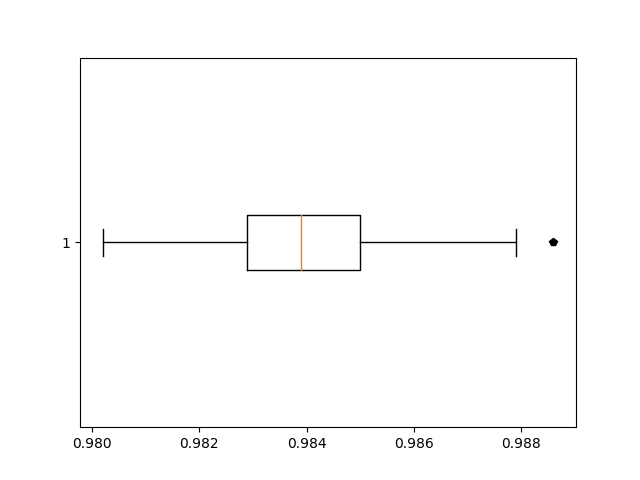
\includegraphics[width=0.50\textwidth]{results/resistor_boxplot}
\end{wrapfigure}

\lipsum[1]


\begin{wrapfigure}{l}{0.50\textwidth}
    \centering
    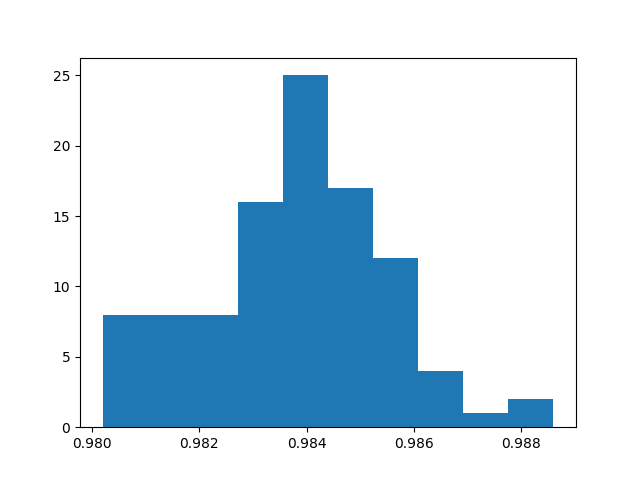
\includegraphics[width=0.50\textwidth]{results/resistor_histogram}
\end{wrapfigure}

\lipsum[2-3]

\newpage

\subsection*{Set Two}
\addcontentsline{toc}{subsection}{Set Two}

\lipsum[4]

\begin{comment}
    Report requirements:
    - Define all notation
    - Include descriptions of tables, figures
    - Take writing to UTA Writing Center
    
    Includes:
    - Cover page
    - - Complete, includes nec. info 
    - Data section
    - - Describe data collection process
    - - - Enough info for someone to replicate process
    - Descriptive Statistics
    - - Include results from descriptive analysis
    - - Interpret results of:
    - - - Box-and-whisker plot
    - - - Histogram
    - - Do sets follow distributions? 1/2 = normal/exponential dist?
    - Appendices I/II:
    - - Tables of raw data for each set
    - - Code
    - - Equipment used
    
    Structure:
    - cover
    - table of contents
    - body
    - - motivation
    - - the data 
    - - collection process
    - - descriptive statistics
    - - methodologies
    - - - tech used (reference appendece for code/tech used)
    - - results 
    - - - figs
    - - answer questions
    - appendices
    - - 1 - set 1 data
    - - 2 - set 2 data
    - - 3 - main analysis code
    - - 4 - helper / preprocessing
    - - 5 - table of equipment

\end{comment}



%-------------------------------------------------------------------------------
% REFERENCES
%-------------------------------------------------------------------------------
\newpage
\section*{References}
\addcontentsline{toc}{section}{References}

Weiss, S., 1989. Tissue Destruction by Neutrophils, \textit{New England Journal of Medicine,} 320, pp. 365-376.
\newline
\newline


\end{document}

%-------------------------------------------------------------------------------
% SNIPPETS
%-------------------------------------------------------------------------------

%\begin{figure}[!ht]
%	\centering
%	\includegraphics[width=0.8\textwidth]{file_name}
%	\caption{}
%	\centering
%	\label{label:file_name}
%\end{figure}

%\begin{figure}[!ht]
%	\centering
%	\includegraphics[width=0.8\textwidth]{graph}
%	\caption{Blood pressure ranges and associated level of hypertension (American Heart Association, 2013).}
%	\centering
%	\label{label:graph}
%\end{figure}

%\begin{wrapfigure}{r}{0.30\textwidth}
%	\vspace{-40pt}
%	\begin{center}
%		\includegraphics[width=0.29\textwidth]{file_name}
%	\end{center}
%	\vspace{-20pt}
%	\caption{}
%	\label{label:file_name}
%\end{wrapfigure}

%\begin{wrapfigure}{r}{0.45\textwidth}
%	\begin{center}
%		\includegraphics[width=0.29\textwidth]{manometer}
%	\end{center}
%	\caption{Aneroid sphygmomanometer with stethoscope (Medicalexpo, 2012).}
%	\label{label:manometer}
%\end{wrapfigure}

%\begin{table}[!ht]\footnotesize
%	\centering
%	\begin{tabular}{cccccc}
%	\toprule
%	\multicolumn{2}{c} {Pearson's correlation test} & \multicolumn{4}{c} {Independent t-test} \\
%	\midrule
%	\multicolumn{2}{c} {Gender} & \multicolumn{2}{c} {Activity level} & \multicolumn{2}{c} {Gender} \\
%	\midrule
%	Males & Females & 1st level & 6th level & Males & Females \\
%	\midrule
%	\multicolumn{2}{c} {BMI vs. SP} & \multicolumn{2}{c} {Systolic pressure} & \multicolumn{2}{c} {Systolic Pressure} \\
%	\multicolumn{2}{c} {BMI vs. DP} & \multicolumn{2}{c} {Diastolic pressure} & \multicolumn{2}{c} {Diastolic pressure} \\
%	\multicolumn{2}{c} {BMI vs. MAP} & \multicolumn{2}{c} {MAP} & \multicolumn{2}{c} {MAP} \\
%	\multicolumn{2}{c} {W:H ratio vs. SP} & \multicolumn{2}{c} {BMI} & \multicolumn{2}{c} {BMI} \\
%	\multicolumn{2}{c} {W:H ratio vs. DP} & \multicolumn{2}{c} {W:H ratio} & \multicolumn{2}{c} {W:H ratio} \\
%	\multicolumn{2}{c} {W:H ratio vs. MAP} & \multicolumn{2}{c} {\% Body fat} & \multicolumn{2}{c} {\% Body fat} \\
%	\multicolumn{2}{c} {} & \multicolumn{2}{c} {Height} & \multicolumn{2}{c} {Height} \\
%	\multicolumn{2}{c} {} & \multicolumn{2}{c} {Weight} & \multicolumn{2}{c} {Weight} \\
%	\multicolumn{2}{c} {} & \multicolumn{2}{c} {Heart rate} & \multicolumn{2}{c} {Heart rate} \\
%	\bottomrule
%	\end{tabular}
%	\caption{Parameters that were analysed and related statistical test performed for current study. BMI - body mass index; SP - systolic pressure; DP - diastolic pressure; MAP - mean arterial pressure; W:H ratio - waist to hip ratio.}
%	\label{label:tests}
%\end{table}
